\documentclass[oneside,doctype=proposal]{tongjithesis}

% 开题报告封面填表日期：重定义日期填空，不修改类文件与版式
% 若需改为其他日期，只改下面的年/月/日数字即可
\renewcommand{\tjdateblank}{\tjnumline{3em}{2026}~年~\tjnumline{2em}{11}~月~\tjnumline{2em}{11}~日}

\tjbibresource{bib/note.bib}

% 技术路线图用到相对定位（below=… of …）
\usetikzlibrary{positioning}

% 让技术路线图紧随正文，不浮动到别处
\usepackage{float}

% 参考文献：会议/文集类条目去掉“[C]//”，改用句点分隔
% （仅影响 inproceedings / incollection，不影响期刊 [J]、专著 [M] 等）
\AtEveryBibitem{%
  \ifboolexpr{ test {\ifentrytype{inproceedings}} or test {\ifentrytype{incollection}} }
    {\clearfield{usera}}{}}
\renewbibmacro*{in:}{\newunit}

% 预印本（arXiv）条目自定义格式：作者. 题名.arXiv:编号, 年份.
% gb7714-2025 把 @preprint 经源映射转成 online + entrysubtype=preprint，
% 这里对 online 驱动按 entrysubtype 分支：preprint 走自定义格式，其余保持原样。
\newbibmacro{online:preprint}{%
  \usebibmacro{bibindex}%
  \usebibmacro{begentry}%
  \usebibmacro{author/editor+others/translator+others}%
  \ifnameundef{namea}{}{\setunit{\labelnamepunct}\newblock}%
  \clearfield{usera}% 去掉 [PP/OL]
  \usebibmacro{title}%
  \setunit{\adddot}%
  \printtext{arXiv:\thefield{eprint}}%
  \setunit{\addcomma\space}%
  \printfield{year}%
  \addperiod
  \usebibmacro{finentry}}
\newbibmacro{online:standard}{%
  \usebibmacro{bibindex}%
  \usebibmacro{begentry}%
  \usebibmacro{author/editor+others/translator+others}%
\ifnameundef{namea}{}{\setunit{\labelnamepunct}\newblock}%这一段用于去除作者不存在时多出的标点
  \usebibmacro{title}%
  \iftoggle{bbx:gbstrict}{}{%
  \newunit%
  \printlist{language}%
  \newunit\newblock
  \usebibmacro{byauthor}%
  \newunit\newblock
  \usebibmacro{byeditor+others}%
  \newunit\newblock
  \printfield{note}}%
  \newunit
  \printfield{version}%
  \newunit\newblock
  \printlist{institution}%%带括号的日期和不带括号的日期
\iffieldundef{entrysubtype}{\newunit\usebibmacro{modifydate}}
    {\ifboolexpr{test {\iffieldequalstr{entrysubtype}{archive}} or test {\iffieldequalstr{entrysubtype}{letter}} or
    test {\iffieldequalstr{entrysubtype}{report}}}
        {\newunit\usebibmacro{newsdate}}
        {\ifboolexpr{test {\iffieldequalstr{entrysubtype}{dataset}} or test {\iffieldequalstr{entrysubtype}{preprint}}}
          {\usebibmacro{modifydate}}{\newunit\usebibmacro{modifydate}}}}%
\iffieldundef{entrysubtype}{\usebibmacro{online:url+urldate}}
    {\iffieldequalstr{entrysubtype}{report}{\usebibmacro{chapter+pages}\newunit\usebibmacro{url}}
        {\usebibmacro{online:url+urldate}}}%
  \newunit\newblock
  \usebibmacro{doi+cstr}%
  \newunit\newblock
  \iftoggle{bbx:eprint}
    {\usebibmacro{eprint}}
    {}%
  \newunit\newblock
  \usebibmacro{addendum+pubstate}%
  \setunit{\bibpagerefpunct}\newblock
  \usebibmacro{pageref}%
  \newunit\newblock
  \iftoggle{bbx:related}
    {\usebibmacro{related:init}%
     \usebibmacro{related}}
    {}%
  \usebibmacro{annotation}\usebibmacro{finentry}}
\DeclareBibliographyDriver{online}{%
  \ifboolexpr{test {\iffieldequalstr{entrysubtype}{preprint}}}
    {\usebibmacro{online:preprint}}
    {\usebibmacro{online:standard}}}

\begin{document}
\pagestyle{empty}

% ============================================================
%  文档类选项（在 main.tex 的 \documentclass[...]{tongjithesis} 中设置）
%  field=science    理工科（工科类、理科类，默认）— 章节编号：1 / 1.1 / 1.1.1
%  field=humanities 文科  （人文、法学、外语、艺术）        — 章节编号：一、/（一）/ 1.
%  经管类属社科：编号要求依理工，撰写依理工模板；26 届为过渡期，可选 science 或
%  humanities；自 27 届起统一使用 science。
% ============================================================

% ============================================================
%  封面信息
% ============================================================
\school{计算机科学与技术学院}
\major{软件工程}
\student{2351289}{周慧星}
\thesistitle{基于多模态流式感知与时空记忆的\mbox{视觉语言导航研究}}{}
% 英文题名：仅首词与专有名词首字母大写（撰写规范）
\thesistitleeng{Research on vision-and-language navigation based on multimodal streaming perception and spatiotemporal memory}{}
\thesisadvisor{蒋寻\quad 教授}
\thesisdate{\the\year}{\the\month}{\the\day} % 使用当前日期；也可以自定义日期

% 任务书专用信息（仅编译 taskbook.tex 时使用；起始年/月/日、截止年/月/日）
% 周数由起讫日期自动换算（向上取整），无需手动填写
\taskbookperiod{2026}{9}{14}{2027}{4}{28}

% 中期报告“专业审核意见”的同意/不同意复选框（仅编译 midterm.tex 时使用）：
% 默认两格均留空，供打印后手写勾选；如需提前在电子版中标注，取消以下一行注释
% \midtermdecision{agree} % 或 disagree

% ============================================================
%  信息说明页
% ============================================================

% 成果类型（三选一）：
%   thesis      — 毕业论文（摘要页标题：摘要）
%   design      — 毕业设计（软件/创意/建筑等非工程设计类；摘要页标题：摘要）
%   engineering — 毕业设计（工程设计类；摘要页标题：设计总说明）
\infotype{thesis}

% 内容简述（300字以内）
\infoabstract{%
请在此处填写论文内容简述，字数建议不超过300字。内容简述应概括论文的研究背景与问题动机、研究目标、主要方法与技术路线、实验设计与数据来源、关键实验结果及性能指标，以及研究结论与创新点，使读者能够快速了解本论文的核心贡献与研究意义。建议按照以下结构来组织简述内容：首先介绍研究背景与问题动机，充分说明研究的必要性与现有相关工作的主要不足之处；其次阐述所提出的方法或技术方案及其设计原理与主要实现细节；然后给出在典型数据集或实际应用场景下的主要实验结果与量化评价指标的全面横向对比分析；最后总结本研究的主要结论与当前局限性，并展望未来改进方向与潜在应用前景。请将以上示例文字全部替换为您的实际内容简述。
}

% 毕业设计：图纸数量与正文字数（成果类型为 design 或 engineering 时填写，两者须同时填写）
% \infodrawings{5}
% \infowordcount{15000}

% 毕业论文：正文总字数（成果类型为 thesis 时填写）
\infothesiswords{12345}

% 随附资料（每条用 \item 开头；不填则显示空白行）
\infomaterials{
  \item 随附资料名称一（如：全套图纸、程序源代码、计算书等）；
  \item 随附资料名称二
}

% ============================================================
%  中英文摘要页
% ============================================================
% 摘要页论文标题（可选）：设置摘要页展示的论文标题（不是“摘要”二字的标题）。未设置或两个参数都留空时，沿用 \thesistitle 与 \thesistitleeng。如需让摘要页使用不同标题或独立换行位置，取消以下两行注释。
% \abstracttitle{\TongjiThesis{}同济大学本科毕业设计（论文）模板与\LaTeX{}排版技术应用}{模板排版功能示例、学术写作规范与格式设置指南}
% \abstracttitleeng{\TongjiThesis{} template and \LaTeX{} typesetting for Tongji University undergraduate thesis}{A guide to typesetting features, academic writing standards, and formatting}

\MakeDocument
% 开题报告不分章节，图表按全文顺序编号，去掉“0.”前缀
\renewcommand{\thefigure}{\arabic{figure}}
\renewcommand{\thetable}{\arabic{table}}

\tjformsection{一、毕业论文课题背景}

\tjformsubsection{1．课题来源及研究的目的和意义}

\textbf{课题来源：}本课题源自指导教师课题组在视觉语言导航（Vision-and-Language Navigation，VLN）与具身智能方向的研究工作。课题以预训练的视觉语言导航模型（如以 Qwen2.5-VL 为底座的 StreamVLN）和连续环境仿真平台（Habitat 及 R2R-CE、RxR-CE 数据集）为基础，研究流式导航中的多模态感知注入与有界时空记忆组织方法，主要参考 StreamVLN、MapNav、NaVid 等代表性工作。

\textbf{研究目的：}VLN 要求智能体依据自然语言指令，在未知三维环境中自主到达目标，是连接语言理解、环境感知与机器人决策的基础任务\cite{anderson2018vln}。随着视觉语言大模型的发展，研究重心已从离散可视图上的“选节点”转向连续环境中“在线接收视觉流并即时决策”，后者也更接近真实机器人的运行条件\cite{krantz2020vlnce,zhang2024navid}。

然而，现有流式方法的能力仍主要来自 RGB 语义。对代表性模型的实现进行核查后发现：模型接收了深度与位姿，却未将其用于前向计算；历史帧仅按等间隔拼接，既无空间去重，也无容量约束，上下文随重复观测不断膨胀；记忆 token 削减 35\% 时，单次前向仅加快 4.1\%，二者不成比例。因此，在冻结主体参数的前提下，如何重新设计输入上下文的内容与组织方式，成为亟待解决的问题。

据此，本课题拟研究多模态流式感知与有界时空记忆驱动的 VLN 方法，目标有三：一是建立严格因果的在线输入与统一评测框架；二是通过语义层与执行层以训练无关的方式将几何与运动状态注入决策，并考察经小型投影层的特征层注入；三是设计规模有界的时空记忆，并通过可分离混杂因素的对照实验，定量刻画视觉、几何、运动与记忆四类信息的边际贡献与代价。

\textbf{研究意义：}方法上，本课题不追求新的端到端模型，而是在冻结权重的条件下考察各类信息的贡献，并给出可证伪的对照协议，有助于厘清流式导航的能力来源；工程上，方案以结构化字段与有界缓存实现，除特征层的小型投影层外不增加参数，在单卡上即可验证与迁移；评测上，同步记录精度与在线开销，使精度与效率的权衡可以得到检验，而不是作为默认假设。

\tjformsubsection{2．国内外在该方向的研究现状和发展趋势}

\textbf{（1）任务定义与评测基准：}R2R 建立了“指令—路径”配对的离散图导航范式，并确立了成功率（SR）、成功加权路径长度（SPL）与导航误差（NE）等指标\cite{anderson2018vln}。VLN-CE 将同一批指令迁移至连续环境，并建立在 Habitat 仿真平台之上\cite{krantz2020vlnce,savva2019habitat}；Waypoint 模型表明，连续环境中可直接回归局部路点，而无需依赖可视图\cite{krantz2021waypoint}。RxR 引入多语言指令与稠密时空标注，并补充了 nDTW、SDTW 等路径对齐指标\cite{ku2020rxr,ilharco2019ndtw}。仅以终点是否可达为判据，无法区分“到达目标”与“按指令所指路线到达”。此外，HM3D 等大规模场景数据为场景泛化研究提供了条件\cite{ramakrishnan2021hm3d}。

\textbf{（2）视频视觉语言模型直接导航：}NaVid 验证了视频 VLM 可依据连续画面与指令直接输出导航动作，且无需建图与深度输入\cite{zhang2024navid}；Uni-NaVid 将导航、目标跟踪与视觉问答统一于同一个视觉—语言—动作模型\cite{zhang2025uninavid}；NaVILA 将“去哪里”与“怎么走”解耦，由高层输出语言化动作，再由低层运动策略执行\cite{cheng2025navila}；NavGPT 利用大模型的显式推理能力进行子目标分解\cite{zhou2024navgpt}。这些方法的共同运行前提是“向强模型提供足够多的视觉历史”，其代价是上下文随回合长度增长，而性能收益是否来自历史本身，仍缺少等预算对照。

\textbf{（3）流式上下文与记忆机制：}StreamVLN 采用快慢双上下文：近期帧保留细节，历史帧经三维感知压缩后写入记忆槽位\cite{wei2025streamvln}；MapNav 以带标注的语义地图替代历史图像，将记忆显式化为可检索的空间结构\cite{zhang2025mapnav}。推理侧也有相邻进展：StreamingLLM 以注意力汇点维持流式生成\cite{xiao2024streamingllm}，FastV 在浅层裁减图像 token\cite{chen2024fastv}。二者分别作用于 KV 状态与视觉 token 两个层次，现有工作多只覆盖其中一类，也较少在等 token 预算下进行横向比较。本课题前期实测表明，二者并不等价：削减外部缓存可降低注意力流量，却几乎不改变单次前向的主要成本。

\textbf{（4）多模态几何与机器人状态：}深度与点云在机器人导航中已被广泛使用。在 VLN 中，几何信息或以深度图作为额外观测通道，或由深度反投影构建局部点云与占据栅格，或以可通行性预测辅助决策；但这些做法多以辅助通道或训练期监督的形式出现，在推理阶段显式使用的情形有限。机器人自身的执行状态（指令动作与实际位移的偏差、是否受阻）则更少进入决策回路，而这类信息恰能指出环境未执行已下发指令的情形，这正是连续环境中重复无效动作的直接来源。

\textbf{（5）效率与评测规范：}连续导航的在线延迟取决于决策频率与单次前向成本的乘积，而非仅由视觉 token 数量决定。前期实测显示：动作分块长度在训练时已固定，若主动缩短每次前向所执行的动作数，总耗时将上升一倍以上，而延迟对 token 削减的弹性仅约 0.11。因此，近期研究逐渐将延迟、显存峰值、token 开销与前向次数同精度一并报告，并要求区分首次调用、稳态与模型加载三个阶段。

\textbf{（6）发展趋势与本课题的切入点：}综合来看，该方向呈现四点趋势：由离散图走向连续环境；由单帧观测走向流式长视频；由单一 RGB 走向“视觉—几何—状态”的多模态融合；由只报精度走向精度与效率并重。对照上述趋势并复核代表性方法的公开实现，可归纳出两个尚待解决的问题：一是几何与运动信息在流式推理中尚未真正参与决策，模型仍主要依赖视觉语义；二是历史信息以无去重的特征拼接方式注入，记忆规模与内容缺少显式约束，且已有压缩手段的收益尚未拆解到精度、延迟与 token 三个维度。

\tjformsection{二、毕业论文方案介绍}

\tjformsubsection{1．主要研究内容}

本课题的预期研究目标如下：建立严格因果的流式输入与统一评测框架；提出空间状态的分层表征与注入方式，其中语义层与执行层训练无关，特征层仅训练小型投影层；提出规模有界的时空记忆组织与空间冗余剪枝方法；在公开连续导航基准上完成对照、消融与鲁棒性实验，给出精度与效率的联合分析，并形成可复现的程序、配置与实验记录。

围绕上述目标，研究内容包括以下五项。

\begin{enumerate}
  \item \textbf{因果流式输入与统一评测框架。}研究 R2R-CE 与 RxR-CE 的数据组织、指令形式、观测与评测方式，建立以时间戳为约束的在线输入流程：决策仅接收不晚于当前时刻的样本，乱序、越界与跨回合观测一律拒绝。同时，建立统一的指标与开销记录体系，使精度与效率在同一口径下可比。
  \item \textbf{视觉流式基线与历史组织分析。}以代表性流式模型为基础，构建单帧、固定窗口与历史流等不同历史组织方式的基线，分别考察历史长度、决策更新频率与缓存策略对导航精度与推理效率的影响，从而明确后续改进的边界条件与成本瓶颈。
  \item \textbf{空间状态的多层级表征与注入。}由深度导出局部几何，由位姿与已下发动作导出运动状态，并将同一份状态分三层注入：以定长结构化字段进入上下文（语义层）；在动作执行前参与可行性否决与卡死恢复（执行层）；将深度反投影为三维 token，经小型投影层并入视觉序列（特征层）。前两层训练无关，特征层仅训练投影层，用于考察模型能否在表征层面利用几何信息。
  \item \textbf{有界时空记忆与空间冗余剪枝。}针对历史冗余、上下文增长与空间重复观测等问题，研究近期窗口与长期缓存的分层组织、基于位置网格的空间去重与检索策略，以及将历史视觉特征按深度反投影到体素后合并的剪枝方法，使记忆规模与输入预算均有界。
  \item \textbf{对照、消融、鲁棒性与效率实验。}设计可分离信息内容、输入长度与执行扰动的对照组，在两个基准上开展主实验、消融实验与感知退化条件下的鲁棒性实验，并对结果进行配对统计检验与误差分析。
\end{enumerate}

\tjformsubsection{2．研究方案}

\textbf{（1）总体技术路线。}研究按“输入—表征—注入—决策—记忆—评测”六个环节展开，如图 1 所示：输入层负责时间戳校验与因果筛选；表征层在保留基线视觉窗口的同时，将深度与位姿压缩为定长结构化量；注入层将同一份状态分别送入语义、执行与特征三个通道；决策层采用参数冻结的流式视觉语言导航模型；记忆层由近期窗口与长期缓存组成，作用于表征层；评测层统一记录精度与开销。整条链路不改变模型主体，可训练部分仅限特征通道的投影层。

\begin{figure}[H]
  \centering
  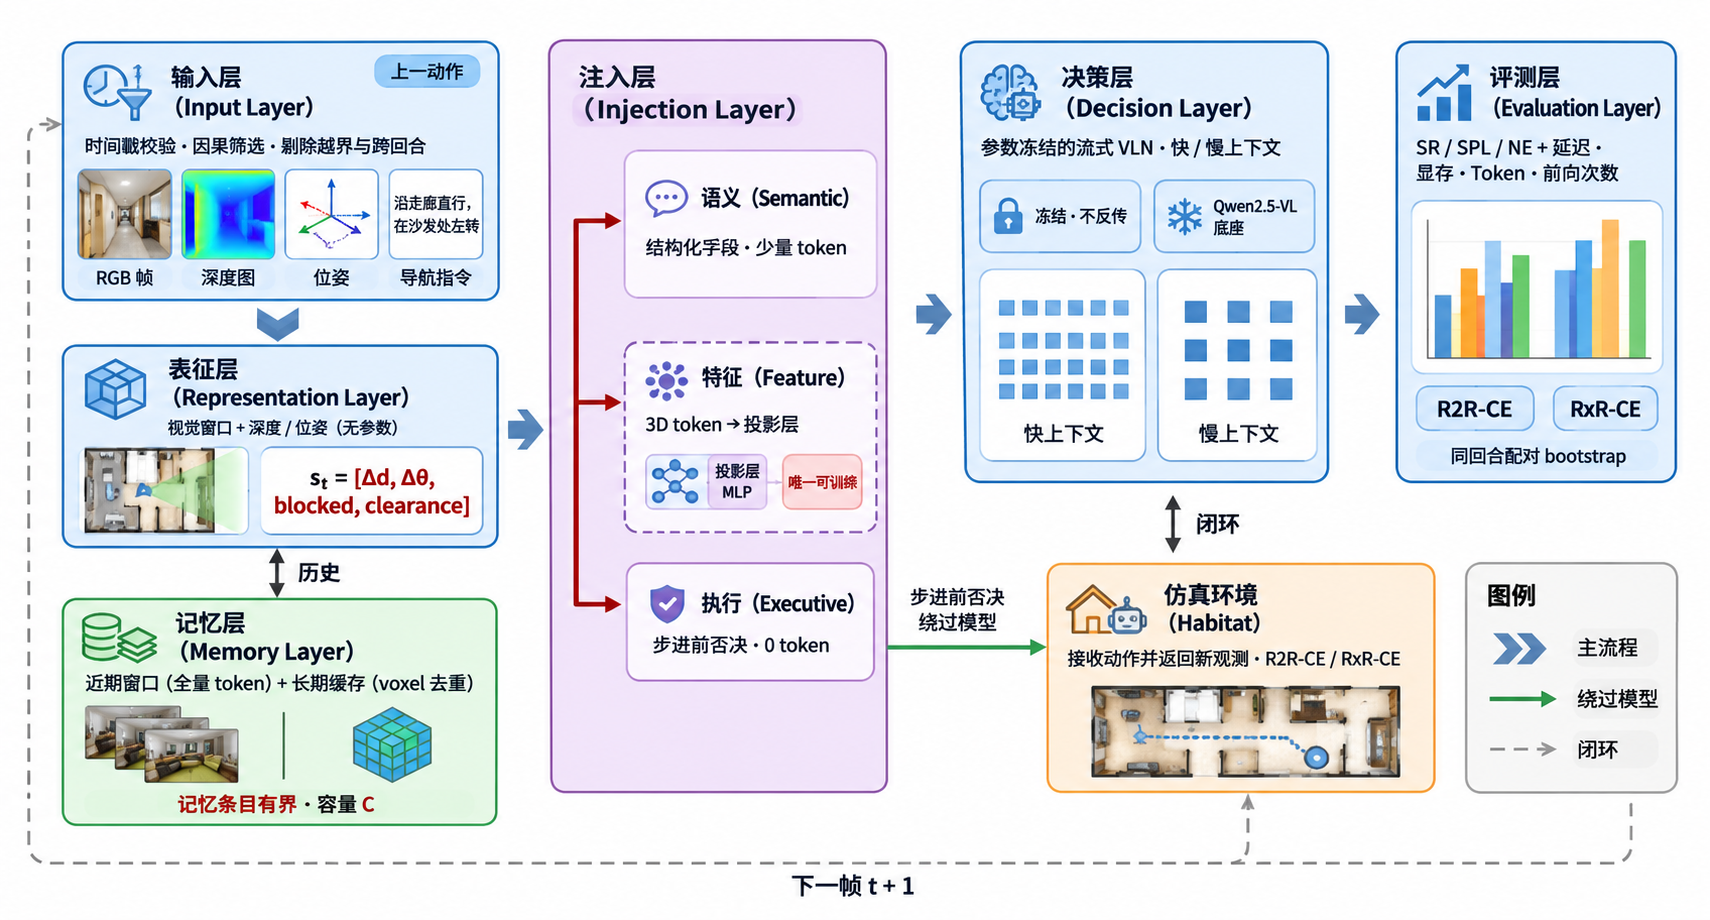
\includegraphics[width=0.9\textwidth]{figures/vln-pipeline-architecture.png}
  \caption{技术路线}
\end{figure}

\textbf{（2）因果流式输入与评测口径。}各传感器观测统一记录采集时刻，决策仅使用不晚于该时刻的样本；乱序、越界与跨回合数据一律拒绝；缺失深度按“未知”处理，不解释为可通行；每回合独立清空记忆与模型状态。评测在 R2R-CE 与 RxR-CE 上开展，除 SR、SPL、NE 外，还逐回合记录推理延迟、显存峰值、输入 token 与前向次数，使精度与效率在同一口径下可比。

\textbf{（3）空间状态的多层级表征与注入。}几何侧由深度反投影得到局部可通行描述，补充单帧图像难以给出的距离与通行性信息；运动侧由位姿与已下发动作得到位移、转角与受阻标记，为碰撞与滑移提供反馈。二者构成同一份定长状态，该状态不引入可训练参数，也不保证障碍的完整性。注入分三层：语义层将状态写成结构化字段，插入指令与动作请求之间，供模型参考但不改变执行；执行层在环境步进前否决不可通行方向，并在卡滞时触发恢复转向，该层不消耗 token，但会改变动作分布；特征层将三维点经小型投影层映射为 token，并与视觉 token 拼接，使几何以表征形式参与推理，该层是唯一需要训练的环节，模型主体仍保持冻结。三层增益的来源可能不同，须分别评估。

\textbf{（4）有界时空记忆。}记忆由近期窗口与长期缓存组成：近期窗口保留最新若干帧以维持短期连续性；淘汰出窗口的观测写入长期缓存，缓存以位置网格为键，同一网格只保留最近一条，容量已满时按最久未更新原则淘汰；检索时先按标签与指令的匹配程度排序，再按时间次序排列，并限制单次检索条数。由此，历史记录数与模型可见条目数均有界。在此基础上，于特征层面再按深度将历史特征反投影到体素，并合并落入同一体素的 token，使记忆规模随重复观测收敛，而不随回合长度线性增长。

\textbf{（5）实验设计与评价。}实验按信息集合分组：以纯视觉为基准，逐步加入几何与运动状态，并设置仅执行通道、等长占位符与随机否决等对照，以区分增益来源；特征层设置等预算对照，以区分几何信息与序列变长各自的贡献。各组使用相同的回合集合与随机种子，并以同回合配对的 bootstrap 区间而非跨样本均值作为判据。记忆部分设置等预算对照与容量扫描，并按路径与指令长度分箱，考察长时收益；鲁棒性实验在感知侧施加光照、深度与位姿扰动，且扰动仅作用于已观测数据。除平均指标外，还同时观察卡死回合比例与前向次数，作为闭环有效性的旁证。

\textbf{（6）可行性。}方法上，本课题不训练模型主体，改进集中于输入组织、上下文构造与小型投影层，算力需求低、风险可控；几何与状态的提取为确定性计算，结果可解释、可复现。条件上，连续导航的场景数据、标注与官方权重均已就位，Habitat 环境与评测链路已在单卡上跑通，基线指标与原文报告值接近，具备开展对照实验的直接条件。实现上，几何与状态模块独立于模型，可单独开关和替换，便于逐项归因。

\textbf{（7）存在的困难与应对。}一是算力有限，全量评测成本较高，拟以固定子集开展主要对照，必要时再补充全量验证。二是几何信息的作用可能有限，仅以文本描述几何的收益并不稳定，故将几何按语义、执行、特征三层分别检验，并接受负结果。三是特征层需要少量训练，而单卡条件下训练规模受限；拟先以零训练方式验证模型能否直接接受三维 token，再决定是否引入投影层训练与对齐损失，若收益不足则退回前两层。四是位姿取自仿真中的理想定位，与真实里程计存在差距，拟将位姿噪声作为独立因素加以考察，不宣称已具备实机定位能力。

\tjformsubsection{3．工作进度安排}

\begin{table}[H]
  \centering
  \caption{工作进度安排}
  \begin{tabularx}{\textwidth}{@{}l X@{}}
    \toprule
    周次 & 主要工作 \\
    \midrule
    第 1—4 周   & 开展视觉语言导航、连续环境导航、视觉语言大模型、多模态感知及流式记忆相关文献调研，熟悉 R2R-CE、RxR-CE 和 Habitat 等数据与平台，明确研究问题和实验设定，完成开题准备。 \\
    第 5—8 周   & 搭建实验环境，完成数据预处理和传感器观测读取流程，复现或运行代表性的 VLN/VLM 模型，建立基于视觉输入的导航基线和统一评测脚本。 \\
    第 9—12 周  & 将基础模型整理为严格因果的流式推理模式，构建单帧、固定窗口和历史流输入等基线，分析历史长度、更新频率以及缓存策略对导航精度和推理效率的影响。 \\
    第 13—18 周 & 研究多模态流式感知与轻量级融合方案，引入深度/局部点云、可通行空间及机器人位姿/运动状态，完成“视觉+几何”“视觉+几何+状态”等主要方案；并尝试将三维 token 经小型投影层并入视觉序列，开展初步实验。 \\
    第 19—24 周 & 研究短时上下文与长期时空记忆机制，探索滑动窗口、特征缓存、KV 缓存、基于三维位置的空间裁剪或语义—几何记忆等方法，完成主要方法设计及核心实验。 \\
    第 25—27 周 & 补充不同数据集、不同历史长度和不同模态组合下的对比实验与消融实验，分析感知退化、几何噪声或里程计扰动等条件下的鲁棒性，并视条件探索真实机器人扩展。 \\
    第 28—30 周 & 整理实验结果、方法结构图及分析图表，完成毕业论文初稿，并整理代码、配置文件和复现实验说明。 \\
    第 31—32 周 & 根据指导意见修改完善毕业论文，完成最终材料提交和毕业答辩准备。 \\
    \bottomrule
  \end{tabularx}
\end{table}

\tjformsection{三、毕业论文的主要参考文献}

\printbibliography[heading=none]

% 封面“填表日期”沿用编译日期；审核意见栏的签名日期由教师手写，故恢复为空白填空
\renewcommand{\tjdateblank}{\ulinebox{3em}~年~\ulinebox{2em}~月~\ulinebox{2em}~日}

\tjformsection{四、审核意见}

\begin{tjreviewbox}
  \tjformlabel{指导教师意见：}\tjformhint{（课题难度是否适中、工作量是否饱满、进度安排是否合理、工作条件是否具备、是否同意开题等）}

  \vspace{8\baselineskip}
  \tjformsignature{指导教师签名}{8em}
\end{tjreviewbox}

\begin{tjreviewbox}
  \tjformlabel{专业审核意见：}\tjformhint{（适当对各项内容给予意见和评价，字数不限。）}

  \vspace{6\baselineskip}
  \tjformsignature{负责人签名}{8em}
\end{tjreviewbox}


\end{document}
